%TC:envir minted 1 xall 
%TC:envir algorithmic 1 xall

% Include tables in word count
%TC:envir table 0 word
%TC:envir tabular 1 word

% Include footnotes in word count
%TC:macro \footnote [text]
%TC:macro \footnotetext [text]

%TC:group minted 0 0
%TC:macro \mintinline [ignore]
%TC:macro \colb [ignore]
%TC:macro \hyperref [ignore]

You will need three Raspberry Pis: two acting as hosts and one as the router. You will also need two Ethernet cables and two USB-to-Ethernet adapters. Use the cables to connect both your hosts to the router as shown below. Static router addresses have been defined by the P4 program.

\begin{figure}[htbp]
  \centering
    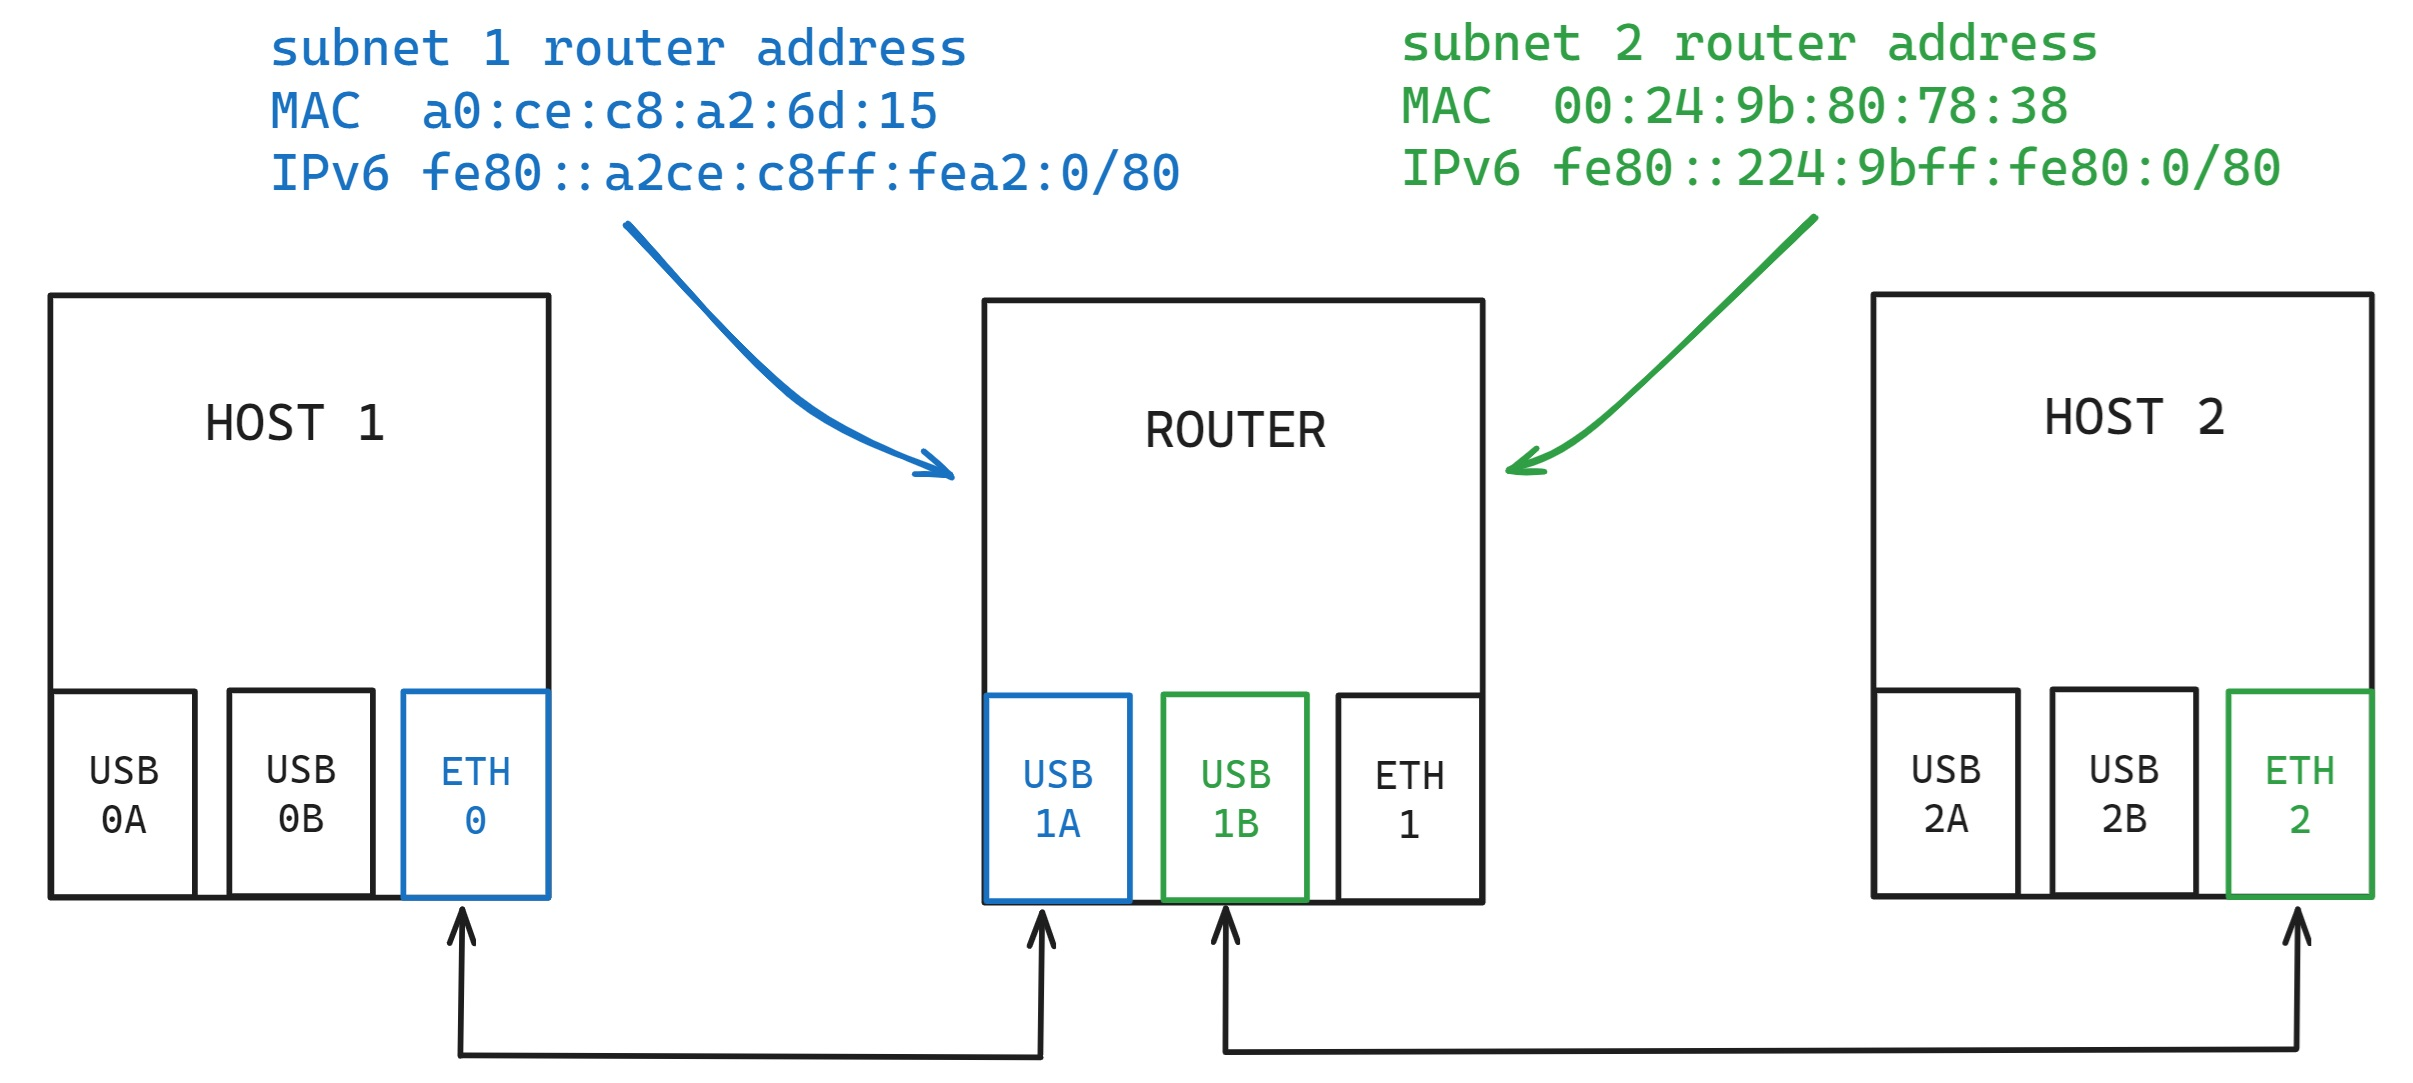
\includegraphics[width=1\textwidth]{figures/appendices/icmpv6_ndp_setup.jpg}
\end{figure}

Run \texttt{ip a} on the router to learn the MAC and IP addresses of the USB ports connected to your hosts. Edit the P4 program to define constant static router IPv6 and MAC addresses (at the top of the program) such that you have one entry for each subnet. These will be referred to as \texttt{IPra}, \texttt{MACra} and \texttt{IPrb}, \texttt{MACrb}. The MAC addresses should match the router’s port MAC addresses, and the IP addresses should belong to the same subnets as the ports. 

Choose IPv6 addresses \texttt{IPa} and \texttt{IPb} for the hosts such that they belong to the same subnet as their respective router USB ports. Also run \texttt{ip a} on the hosts to learn their MAC addresses \texttt{MACa} and \texttt{MACb}.

On Host 1, open a command prompt and run:
\begin{quote}
    \texttt{sudo ifconfig eth0 inet6 add IPa}
    
    \texttt{sudo ip -6 route add dev eth0 IPra}
    
    \texttt{sudo ip -6 neigh add dev eth0 IPra lladdr MACra}
\end{quote}

The first line sets a static IPv6 address on Host 1, the second line defines a route to the static address and the third line puts an entry in Host 1’s neighbour table, associating the router IPv6 address with the specified router MAC address.

Run the same commands on Host 2:
\begin{quote}
    \texttt{sudo ifconfig eth0 inet6 add IPb}
    
    \texttt{sudo ip -6 route add dev eth0 IPrb}
    
    \texttt{sudo ip -6 neigh add dev eth0 IPrb lladdr MACrb}
\end{quote}

Start the P4 program on the router using the port connected to Host 1. Then, run the \texttt{ping} command on Host 1:
\begin{quote}
    \texttt{ping6 -I eth0 IPra}
\end{quote}

Or on Host 2: 
\begin{quote}
    \texttt{ping6 -I eth0 IPrb}
\end{quote}

These should generate an Echo Reply from the respective router addresses. To receive a Time Exceeded error message, use an additional argument to set the hop limit to 1, e.g.:
\begin{quote}
    \texttt{ping6 -I eth0 IPra -t 1}
\end{quote}

If you define a route and MAC neighbour entry to a random address and then direct an Echo Request towards it, you should receive a Destination Unreachable error message from the router.
